\documentclass{standalone}
\usepackage{tikz}
\usetikzlibrary{patterns}
\usetikzlibrary{positioning}
\usetikzlibrary{patterns, positioning}
\usetikzlibrary{shapes.misc}
\usepackage[outline]{contour}
\contourlength{1.5pt} 
\usepackage[sfdefault]{ClearSans}

\begin{document}
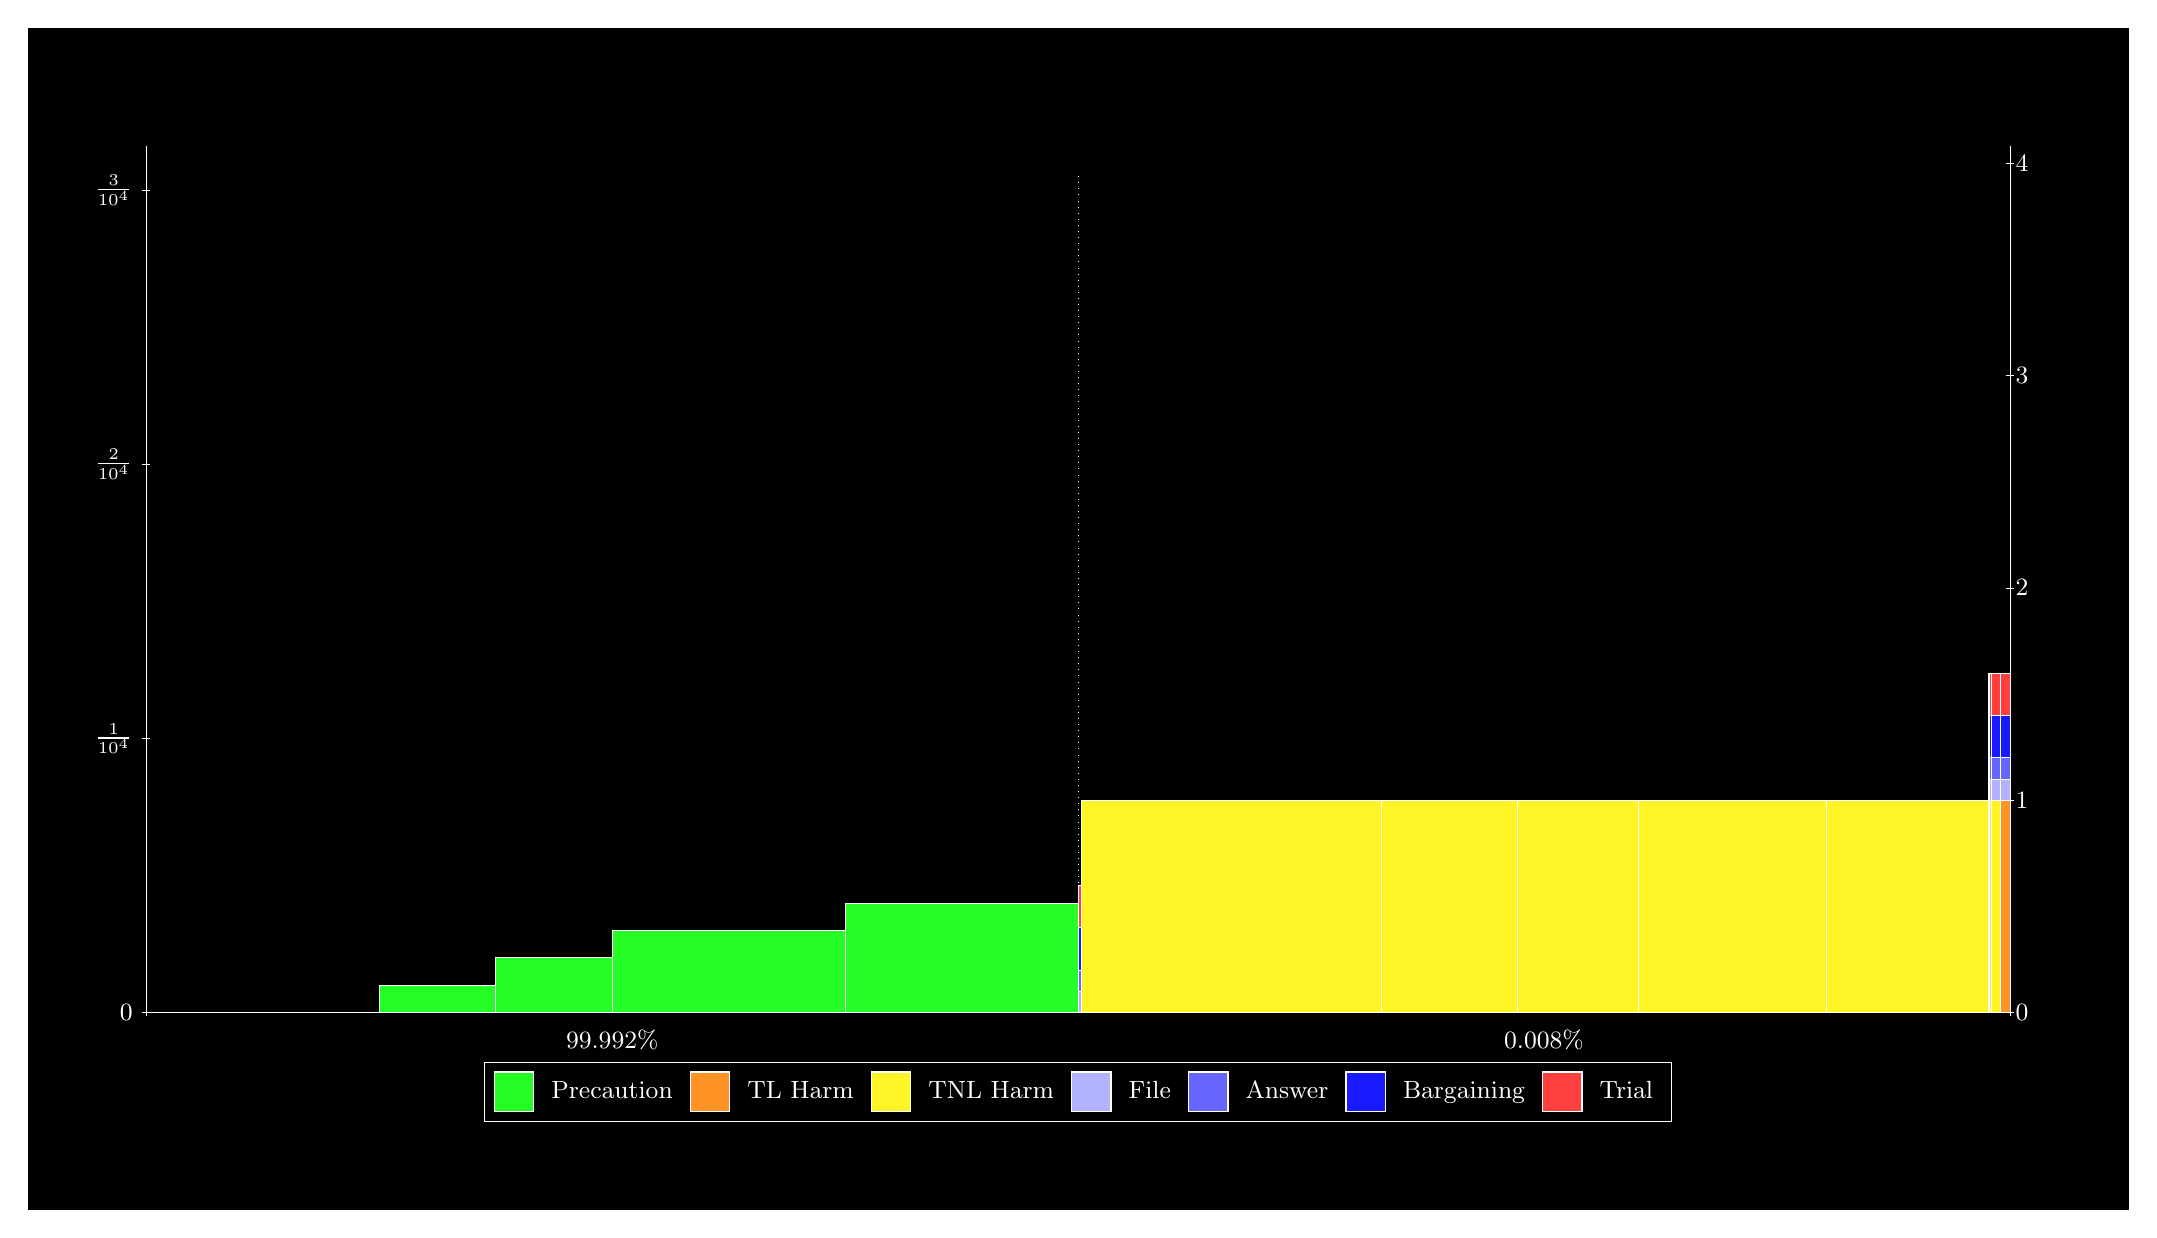
\begin{tikzpicture}
\draw[fill=black] (0,0) rectangle (26.667,15);
\draw[fill=green!85,draw=white,very thin] (4.4582,2.5) rectangle (5.9374,2.8481);
\draw[fill=green!85,draw=white,very thin] (5.9374,2.5) rectangle (7.4166,3.1963);
\draw[fill=green!85,draw=white,very thin] (7.4166,2.5) rectangle (10.375,3.5444);
\draw[fill=green!85,draw=white,very thin] (10.375,2.5) rectangle (13.333,3.8925);
\draw[fill=green!85,draw=white,very thin] (13.333,2.5) rectangle (13.369,2.5001);
\draw[fill=blue!30,draw=white,very thin] (13.333,2.5001) rectangle (13.369,2.7697);
\draw[fill=blue!60,draw=white,very thin] (13.333,2.7697) rectangle (13.369,3.0393);
\draw[fill=blue!90,draw=white,very thin] (13.333,3.0393) rectangle (13.369,3.5786);
\draw[fill=red!75,draw=white,very thin] (13.333,3.5786) rectangle (13.369,4.1178);
\draw[fill=yellow!85,draw=white,very thin] (13.369,2.5) rectangle (17.185,5.1963);
\draw[fill=green!85,draw=white,very thin] (17.185,2.5) rectangle (18.91,2.5);
\draw[fill=yellow!85,draw=white,very thin] (17.185,2.5) rectangle (18.91,5.1963);
\draw[fill=green!85,draw=white,very thin] (18.91,2.5) rectangle (20.446,2.5001);
\draw[fill=yellow!85,draw=white,very thin] (18.91,2.5001) rectangle (20.446,5.1963);
\draw[fill=green!85,draw=white,very thin] (20.446,2.5) rectangle (22.832,2.5001);
\draw[fill=yellow!85,draw=white,very thin] (20.446,2.5001) rectangle (22.832,5.1963);
\draw[fill=green!85,draw=white,very thin] (22.832,2.5) rectangle (22.841,2.5001);
\draw[fill=orange!85,draw=white,very thin] (22.832,2.5001) rectangle (22.841,5.1963);
\draw[fill=green!85,draw=white,very thin] (22.841,2.5) rectangle (24.888,2.5001);
\draw[fill=yellow!85,draw=white,very thin] (22.841,2.5001) rectangle (24.888,5.1964);
\draw[fill=yellow!85,draw=white,very thin] (24.888,2.5) rectangle (24.892,5.1963);
\draw[fill=blue!30,draw=white,very thin] (24.888,5.1963) rectangle (24.892,5.4659);
\draw[fill=blue!60,draw=white,very thin] (24.888,5.4659) rectangle (24.892,5.7355);
\draw[fill=blue!90,draw=white,very thin] (24.888,5.7355) rectangle (24.892,6.2748);
\draw[fill=red!75,draw=white,very thin] (24.888,6.2748) rectangle (24.892,6.814);
\draw[fill=green!85,draw=white,very thin] (24.892,2.5) rectangle (24.911,2.5);
\draw[fill=yellow!85,draw=white,very thin] (24.892,2.5) rectangle (24.911,5.1963);
\draw[fill=blue!30,draw=white,very thin] (24.892,5.1963) rectangle (24.911,5.4659);
\draw[fill=blue!60,draw=white,very thin] (24.892,5.4659) rectangle (24.911,5.7355);
\draw[fill=blue!90,draw=white,very thin] (24.892,5.7355) rectangle (24.911,6.2748);
\draw[fill=red!75,draw=white,very thin] (24.892,6.2748) rectangle (24.911,6.814);
\draw[fill=green!85,draw=white,very thin] (24.911,2.5) rectangle (24.928,2.5001);
\draw[fill=yellow!85,draw=white,very thin] (24.911,2.5001) rectangle (24.928,5.1963);
\draw[fill=blue!30,draw=white,very thin] (24.911,5.1963) rectangle (24.928,5.4659);
\draw[fill=blue!60,draw=white,very thin] (24.911,5.4659) rectangle (24.928,5.7356);
\draw[fill=blue!90,draw=white,very thin] (24.911,5.7356) rectangle (24.928,6.2748);
\draw[fill=red!75,draw=white,very thin] (24.911,6.2748) rectangle (24.928,6.8141);
\draw[fill=green!85,draw=white,very thin] (24.928,2.5) rectangle (25.045,2.5001);
\draw[fill=yellow!85,draw=white,very thin] (24.928,2.5001) rectangle (25.045,5.1963);
\draw[fill=blue!30,draw=white,very thin] (24.928,5.1963) rectangle (25.045,5.466);
\draw[fill=blue!60,draw=white,very thin] (24.928,5.466) rectangle (25.045,5.7356);
\draw[fill=blue!90,draw=white,very thin] (24.928,5.7356) rectangle (25.045,6.2748);
\draw[fill=red!75,draw=white,very thin] (24.928,6.2748) rectangle (25.045,6.8141);
\draw[fill=green!85,draw=white,very thin] (25.045,2.5) rectangle (25.167,2.5001);
\draw[fill=orange!85,draw=white,very thin] (25.045,2.5001) rectangle (25.167,5.1963);
\draw[fill=blue!30,draw=white,very thin] (25.045,5.1963) rectangle (25.167,5.466);
\draw[fill=blue!60,draw=white,very thin] (25.045,5.466) rectangle (25.167,5.7356);
\draw[fill=blue!90,draw=white,very thin] (25.045,5.7356) rectangle (25.167,6.2748);
\draw[fill=red!75,draw=white,very thin] (25.045,6.2748) rectangle (25.167,6.8141);
\draw[white,very thin] (1.5,2.5) -- (1.5,13.5);
\draw[white,very thin] (1.45,2.5) -- (1.55,2.5);
\node[font=\small,text=white, anchor=east] at (1.45, 2.5) {0};
\draw[white,very thin] (1.45,5.9813) -- (1.55,5.9813);
\node[font=\small,text=white, anchor=east] at (1.45, 5.9813) {$\frac{1}{10^{4}}$};
\draw[white,very thin] (1.45,9.4627) -- (1.55,9.4627);
\node[font=\small,text=white, anchor=east] at (1.45, 9.4627) {$\frac{2}{10^{4}}$};
\draw[white,very thin] (1.45,12.944) -- (1.55,12.944);
\node[font=\small,text=white, anchor=east] at (1.45, 12.944) {$\frac{3}{10^{4}}$};

\draw[white,dotted,very thin] (13.333,2.83) -- (13.333,13.17);
\draw[white,very thin] (25.167,2.5) -- (25.167,13.5);
\draw[white,very thin] (25.117,2.5) -- (25.217,2.5);
\node[font=\small,text=white, anchor=west] at (25.117, 2.5) {0};
\draw[white,very thin] (25.117,5.1963) -- (25.217,5.1963);
\node[font=\small,text=white, anchor=west] at (25.117, 5.1963) {1};
\draw[white,very thin] (25.117,7.8925) -- (25.217,7.8925);
\node[font=\small,text=white, anchor=west] at (25.117, 7.8925) {2};
\draw[white,very thin] (25.117,10.589) -- (25.217,10.589);
\node[font=\small,text=white, anchor=west] at (25.117, 10.589) {3};
\draw[white,very thin] (25.117,13.285) -- (25.217,13.285);
\node[font=\small,text=white, anchor=west] at (25.117, 13.285) {4};

\draw[white,very thin] (1.5,2.5) -- (25.167,2.5);
\draw[white,very thin] (1.5,2.45) -- (1.5,2.55);
\node[font=\small,text=white, anchor=north] at (1.5, 2.45) {};
\draw[white,very thin] (25.167,2.45) -- (25.167,2.55);
\node[font=\small,text=white, anchor=north] at (25.167, 2.45) {};

\node[font=\small,text=white,anchor=south] at (7.4167, 1.9) {99.992\%};
\node[font=\small,text=white,anchor=south] at (19.25, 1.9) {0.008\%};
\draw (13.3333,2.5) node (B) {};
\begin{scope}[align=center]
\matrix[scale=0.5,draw=white,below=0.5cm of B,nodes={draw},column sep=0.1cm]{
\node[rectangle,draw,minimum width=0.5cm,minimum height=0.5cm,fill=green!85]{}; & \node[draw=none,font=\small,text=white]{Precaution}; &
\node[rectangle,draw,minimum width=0.5cm,minimum height=0.5cm,fill=orange!85]{}; & \node[draw=none,font=\small,text=white]{TL Harm}; &
\node[rectangle,draw,minimum width=0.5cm,minimum height=0.5cm,fill=yellow!85]{}; & \node[draw=none,font=\small,text=white]{TNL Harm}; &
\node[rectangle,draw,minimum width=0.5cm,minimum height=0.5cm,fill=blue!30]{}; & \node[draw=none,font=\small,text=white]{File}; &
\node[rectangle,draw,minimum width=0.5cm,minimum height=0.5cm,fill=blue!60]{}; & \node[draw=none,font=\small,text=white]{Answer}; &
\node[rectangle,draw,minimum width=0.5cm,minimum height=0.5cm,fill=blue!90]{}; & \node[draw=none,font=\small,text=white]{Bargaining}; &
\node[rectangle,draw,minimum width=0.5cm,minimum height=0.5cm,fill=red!75]{}; & \node[draw=none,font=\small,text=white]{Trial}; \\\\
};\end{scope}

\end{tikzpicture}
\end{document}